\chapter{Blind Demixing} \label{Chap:demix}
In this chapter, we introduce a fundamental problem known as blind demixing which is the general form of blind deconvolution. 
It arises in different fields such as wireless communication, image processing, statistics and machine learning. 
In blind deconvolution, we observe the convolution of two unknown signals and want to separate them, 
whereas in blind demixing we observe the superposition of multiple unknown convolved signals.
In particular, blind demixing turns out to be a promising approach to support low-latency communication with 
unknown channels by reducing channel signaling overhead. This will be particularly, beneficial in growing applications
of Internet-of-things (IoT).

In this chapter, we study how we can incorporate the beneficial information of decoder
into the signal detector. We formulate an algorithm that tackles blind demixing problem and at the same time
restricts the signals that are mapped from a valid codeword bit sequence. The challenge is how we can restrict to the valid codewords
which live on GF(2) domain and take advantage from them in blind demixing algorithms. In particular we study the Wirtinger Flow algorithm for blind demixing that is shown to 
outperform previously introduced methods \cite{candes2015phase, chen2015solving, ma2017implicit, dong2018nonconvex}. 

We will show that  
the state of the art algorithms for blind demixing can be improved by relying on decoder information.


\section{System Model}
Let $\{.\}^*$, $\{.\}^T$, and $\{.\}^H$ denote conjugate, transpose, and conjugate transpose, respectively.
Let $\mathbf{x}_i=[x_{i,1}\cdots, x_{i,K} ]^T$ be the QAM complex signal vector that the i-th source transmits, where $1\leq i \leq S$. 
Each signal vector $\mathbf{x}_i$ is precoded with a matrix $\mathbf{A}_i \in \mathbb{C} ^{N \times K}$ consisting 
of zero mean Gaussian i.i.d. random variables with variance $1$.
Without loss of generality, we focus on OFDM transmissions by defining $N \times N$ matrix $\mathbf{F}$ and $\mathbf{F}^H$ 
be the $N$-point FFT and IFFT matrix respectively where $\mathbf{F}(m, n)= \frac{1}{\sqrt{N}}e^{-j2\pi(m-1)(n-1)/N}, 1 \leq i , j \leq N$ and $\mathbf{F}\mathbf{F}^H = \mathbf{I}$. 

After precoding, the transmitter takes the IFFT and then adds cyclic prefix
so we can write the output of IFFT for i-th source as $$\mathbf{s}_i  = \mathbf{F}^H\mathbf{A}_i\mathbf{x}_i$$
Let's also show the cyclic prefix added version of $\mathbf{s}_i$ by $\tilde{\mathbf{s}}_i$.
Let's also assume $\mathbf{h}_i = [h_{i,1}\cdots, h_{i,L} ]^T$ to be the unknown multipath channel impulse response for the i-th source with maximum length $L$, $\mathbf{h}_i \in \mathbb{C}^L$.
Therefore we can write the received signal as 

\begin{equation}
\tilde{\mathbf{{y}}} = \sum_{i=1}^{S} \tilde{\mathbf{s}}_i \ast \mathbf{h}_i + \hat{\mathbf{n}}
\end{equation}
Where $\hat{\mathbf{n}}$ in complex Gaussian variable to model the AWGN channel and $\ast$ is a linear convolution. Removing the cyclic prefix
from $\tilde{\mathbf{{y}}}$ to get $\hat{\mathbf{y}}$, we can write an equivalent equation for $\hat{\mathbf{y}}$ based on circular convolution shown by $ \circledast$: 

\begin{equation}
\label{circ}
\hat{\mathbf{y}} =  \sum_{i=1}^{S} \mathbf{s}_i \circledast \mathbf{w}_i + \hat{\mathbf{n}}
\end{equation}

Where $\mathbf{w}_i$ is simply $\mathbf{h}_i$ that is extended with zeros to length $N$, equivalently: 
$\mathbf{w}_i = \mathbf{C}\mathbf{h}_i$ where 


\begin{equation}
\label{real}
\mathbf{C} \in  \mathbb{C} ^{N \times L},  \quad \mathbf{C} =
\begin{bmatrix}
\mathbf{I}_L\\
\mathbf{0}
\end{bmatrix} 
\end{equation}

By taking the FFT of the received signal at the receiver we can write the equivalent of equation (\ref{circ}) in frequency domain
%\begin{equation}
%\begin{aligned}
%\mathbf{y} = \mathbf{F}\hat{\mathbf{y}} + \mathbf{F}\hat{\mathbf{n}} = \sum_{i=1}^{S} \mathbf{F}\mathbf{s}_i \odot  \mathbf{F}\mathbf{w}_i + \hat{\mathbf{n}} \\  
%                                                                                                            = \sum_{i=1}^{S} \mathbf{F} \mathbf{F}^H \mathbf{A}_i\mathbf{x}_i\odot \mathbf{F}\mathbf{C}\mathbf{h}_i + \hat{\mathbf{n}}\\                                    
 %                                        								       = \sum_{i=1}^{S} \mathbf{A}_i\mathbf{x}_i\odot \mathbf{B}\mathbf{h}_i  + \hat{\mathbf{n}}

%\end{aligned}                                                                                                          
%\end{equation}

\begin{equation}
\begin{aligned}
\mathbf{y} = \mathbf{F}\hat{\mathbf{y}} & =  \sum_{i=1}^{S} \mathbf{F}\mathbf{s}_i \odot  \mathbf{F}\mathbf{w}_i  + \mathbf{F} \hat{\mathbf{n}} \\  
      & = \sum_{i=1}^{S} \mathbf{F} \mathbf{F}^H \mathbf{A}_i\mathbf{x}_i\odot \mathbf{F}\mathbf{C}\mathbf{h}_i  + \mathbf{F} \hat{\mathbf{n}}\\   
      & = \sum_{i=1}^{S} \mathbf{A}_i \mathbf{x}_i \odot \mathbf{B} \mathbf{h}_i  + \mathbf{n} 
\end{aligned}
\end{equation}


In which $\odot$ is element-wise product and we define $\mathbf{B} = \mathbf{F}\mathbf{C}$ and $\mathbf{n} = \mathbf{F} \hat{\mathbf{n}}$. Let $\mathbf{b}_j^T$ and $\mathbf{a}_{ij}^T $ 
be the j-th row of $\mathbf{B}$ and $\mathbf{A}_i$ respectively. Therefore, each element of $\mathbf{y}$, $y_j$ where $1 \leq j \leq N$ is:


\begin{equation}
\label{dot}
\begin{aligned}
y_j & =  \sum_{i=1}^{S}\mathbf{a}_{ij}^T~\mathbf{x}_i {\mathbf{b}_j}^T \mathbf{h}_i + n_j\\
      & =  \sum_{i=1}^{S} \mathbf{x}_i ^T \mathbf{a}_{ij} {\mathbf{b}_j}^T \mathbf{h}_i + n_j\\ 
      & =  \sum_{i=1}^{S} {\mathbf{b}_j}^T \mathbf{h}_i \mathbf{x}_i ^T \mathbf{a}_{ij} + n_j
\end{aligned}
\end{equation}

Where $ n_j$ is j-th element of white Gaussian noise vector $\mathbf{n}$.
In order to decode the data vectors $\{\mathbf{x}_i\}_1^S$, without prior knowledge about channel state information (CSI) $\{\mathbf{h}_i\}_1^S$ under additive white gaussian noise (AWGN),
we write the Joint maximum likelihood (ML) estimation  as the following optimization problem:

\begin{equation}
\begin{aligned}
\mathcal{P}_1: \quad &\underset{\{x_i\},\{h_i\}}{\text{min}} \quad G(h_1, \cdots, h_S,x_1, \cdots, x_S)\\
& G(h_1, \cdots, h_S,x_1, \cdots, x_S) = \sum_{j=1}^{N} \mid y_j -  \sum_{i=1}^{S} {\mathbf{b}_j}^T \mathbf{h}_i \mathbf{x}_i ^T \mathbf{a}_{ij} \mid^2            
\end{aligned}
\end{equation}




The problem $\mathcal{P}_1$, is non-convex problem that inherently admits multiple local minima. The existence of local minima is evident from at least the inherent scalar ambiguity 
$\gamma$ in each $\mathbf{h}_i \mathbf{x}_i^T = \gamma \mathbf{h}_i(\gamma^{-1}\mathbf{x}_i)^T$. Blind demixing problem targets recovering $\{\mathbf{x}_i\}_1^S$, without prior knowledge about channel state information (CSI) $\{\mathbf{h}_i\}_1^S$. 

\section{Wirtinger Flow Algorithm}
Wirtinger flow aglorithm is a two stage, iterative algorithm consisting of spectral initialization and vanilla gradient decent update 
procedure without regularization that is proposed to optimize non-convex objective function of $\mathcal{P}_1$  \cite{dong2018nonconvex }.
Specifically, by taking advantage of the gradient of a functions with  complex domain known as Wirtinger derivitives, Candes and coworkers  showed Wirtinger flow algorithm is optimal for phase retrieval \cite{candes2015phase}. 

The key point is we initialize within local basin sufficiently close to the ground-truth in a region that there is no saddle points or local minima.

\begin{figure}[h]
\centering
\includegraphics[scale = 0.6]{figs/wf_localbasin}
\caption{Initial guess that can find the global minimum}
\end{figure}


\subsection{Spectral Initialization}
Let's define matrix $M_i$ to be $M_i := \sum_{j=1}^{N}{y_j} \mathbf{b}_j^T \mathbf{a}_{ij} $, for $i = 1 \cdots S$. Let also $\sigma_1(M_i)$,
$\mathbf{u}_i$ and $\mathbf{v}_i$ be the leading singular value, left singular vector and right singular vector of matrix $M_i$, respectively.
We initialize 

\begin{equation}
\begin{aligned}
\mathbf{h}_i^0 = \sqrt{\sigma_1(M_i)} \mathbf{u}_i\\
\mathbf{x}_i^0 = \sqrt{\sigma_1(M_i)} \mathbf{v}_i
\end{aligned}
\end{equation}


\subsection{Update rule}
For $i = 1, \cdots, S$, $\nabla_{\mathbf{h}_i}G$ and $\nabla_{\mathbf{x}_i}G$ denote the Wirtinger gradient of the error function
$G(.)$ with respect to $\mathbf{h}_i$ and $\mathbf{x}_i$, repectively:


\begin{subequations}
\begin{equation}
\nabla_{\mathbf{h}_i} G = \sum_{j=1}^{N} \bigg(  \sum_{i=1}^{S} {\mathbf{b}_j}^T \mathbf{h}_i \mathbf{x}_i ^T \mathbf{a}_{ij} - y_j \bigg) \mathbf{b}_j^* \mathbf{a}_{ij}^H \mathbf{x}_i^*  \\
\end{equation}
\begin{equation}
\nabla_{\mathbf{x}_i} G = \sum_{j=1}^{N} \bigg(  \sum_{i=1}^{S} {\mathbf{b}_j}^T \mathbf{h}_i \mathbf{x}_i ^T \mathbf{a}_{ij} - y_j \bigg)  \mathbf{a}_{ij}^* \mathbf{b}_j^H  \mathbf{h}_i^*
\end{equation}
\end{subequations}

The Wirtinger flow algorithm updates the $t+1$-th iteration using a stepsize $\eta > 0$ via


\begin{subequations}
\begin{equation}
\label{update}
\mathbf{h}_i^{t+1} = \mathbf{h}_i^{t} - \eta \frac{1}{{\parallel \mathbf{x}_i^{t}\parallel }_2^2} \nabla_{\mathbf{h}_i} G(h_1^t, \cdots, h_S^t,x_1^t, \cdots, x_S^t) 
\end{equation}
\begin{equation}
\mathbf{x}_i^{t+1} = \mathbf{x}_i^{t} - \eta \frac{1}{{\parallel \mathbf{h}_i^{t}\parallel }_2^2} \nabla_{\mathbf{x}_i} G(h_1^t, \cdots, h_S^t,x_1^t, \cdots, x_S^t) \end{equation}
\end{subequations}

For $i = 1, \cdots, S$






\section{Robust Wirtinger flow algorithm}

\subsection{Mapping to valid codewords}

We propose to investigate the effectiveness of code constraints to improve the performance of Wirtinger flow algorithm 
to make it more robust against noise and practical obstacles.
We can do so by providing more information about the structure of $\{\mathbf{x}_i\}_1^S$. We know that $\{\mathbf{x}_i\}_1^S$
are QPSK signals that are mapped from a valid codeword to the complex field. In particular, we want to investigate polar codes that 
are widely used for  forward error correction (FEC) of short data packets such as IoT applications although this approach can
be implemented for any type of code. Without loss of generality, we assume the signal of interest for the receiver is $\mathbf{x}_1$.

Let's denote the mapping between $\mathbf{x}_1$ and the bit vector by 
$$ {\cal \tilde{M}}(\bfb)=[x_{1,1}\cdots, x_{1,K} ]$$
Where  $\bfb = [b_1, b_2, \cdots, b_{2K}]$ itself is a valid codeword produced by the encoder from  
a polar code of rate $R = k_0 / 2K$ is specified by 
$(2K, k_0, \mathcal{I}^c)$, where $2K = 2^n$ is the codeword 
length and $k_0$ is the number of information bits in a 
codeword. We can ideally require $\bfb\in {\cal F}$ where ${\cal F}$ denotes the set of all valid FEC codewords of 
length $2K$. The challenge is how to incorporate this information into the Wirtinger flow algorithm. We suggest to map the 
current solution of WF algorithm at iteration $t$ shown by $\mathbf{x}_1^t$, to the set defined by $$\cal X = \{\mathbf{x} \mid  \cal{\tilde{M}}(\bfb) = \mathbf{x}, \bfb\in {\cal F}\}$$
To do so we can formulate an optimization problem as the following:

\begin{equation}
\begin{aligned}
\mathcal{P}_2: \quad &\underset{\mathbf{x}} {\text{min}} &&\parallel \mathbf{x} - \mathbf{x}_1^t \parallel_2^2\\
                                  &\text{s.t.} &&\mathbf{x} \in \cal X\\
\end{aligned}
\end{equation}

And update $\mathbf{x}_1^t$ with the solution of $\mathcal{P}_2$. We do not have to do this mapping in every iteration since we only want to make sure
the algorithm converges to a solution that satisfies the code constraints. In our simulation that comes later we see that doing the mapping in every 5 
iteration gives an optimum result.

However, the limitation is the constraint in $\mathcal{P}_2$ makes it a non-convex problem that is NP-hard and grows exponentially
with the dimension of codeword size. Therefore,  it would be computationally very expensive to solve $\mathcal{P}_2$ as it is.
To address this issue, we propose to use the relaxed version of polar code constraints that is introduced in \cite{goela2010lp} originally to decode polar codes and 
also it has been shown in \cite{jalali2018joint} that can be incorporated in real/complex field to design a MIMO detector for improved signal detection in various scenarios. 








\subsection{Relaxed Polar Codeword Constraints}

Similar to what we did in previous chapters, we integrate information from the
$\bfb\in {\cal F}$ codeword constraint into $\mathcal{P}_2$ when polar codes are adopted as FEC. 
We can write down the linear coding 
constraints by enforcing all the variables of the 
factor graph to comply with the polytope $\mathcal{P}$, 
i.e. $\mathbf{s} \in \mathcal{P}$ where $\mathbf{s}$ 
denotes all the variables of the factor graph. These
constraints can be incorporated into $\mathcal{P}_2$
as relaxed version of $\bfb \in \cal F$.
Therefore, we can change $\mathcal{P}_2$ to

\begin{equation}
\begin{aligned}
\mathcal{P}_3: \quad &\underset{\mathbf{x}} {\text{min}} &&\parallel \mathbf{x} - \mathbf{x}_1^t \parallel_2\\
                                  &\text{s.t.} &&\cal{\tilde{M}}(\bfb) = \mathbf{x}\\
                                                      &&& \mathbf{s} \in \mathcal{P}\\
\end{aligned}
\end{equation}




Note that all $2K (1 + \log 2K)$ variables in $\mathbf{s}$ are optimization variables in the problem of $\mathcal{P}_3$ and
$\bfb$ is the last column of factor graph variables $\mathbf{s}$. 





\subsection{Redefining the Objective Function}
Finally, to formulate computationally less expensive problem, our first step is to modify 
the objective function by changing the $l_2$ norm
 in $\mathcal{P}_3$ objective function 
to $l_1$ norm metric. This will allow us to classically reformulate the norm minimization
into a linear programming (LP) problem. The $l_1$ norm as an optimization
metric has been applied in 
data analysis and parameter estimation because it is robust 
to impulsive noises and other man-made radio
interferences \cite{cui2006linear}. 



We reformulate $\mathcal{P}_2$ into a LP with
two sets of generalized vector inequalities by introducing slack variables $e_k\ge 0,\, 1 \leq k \leq K$. 
We also define $\mathbf{t}$ to be a vector of these slack variables, i.e. $\mathbf{t} = [t_1, \cdots, t_K]$. Consequently we can modify the optimization problem of $\mathcal{P}_3$ to




\begin{equation}
\begin{aligned}
\label{MILP}
\mathcal{P}_4: \quad &\underset{\mathbf{s}} {\text{min}} && \sum_{k=1}^{K} t_k \\
				 &\text{  s.t.}  && \mathbf{x} \preceq  \mathbf{x}_1^t + \mathbf{t}\\
				                  & &&-\mathbf{x} \preceq  -\mathbf{x}_1^t + \mathbf{t}\\
				                  &&&\cal{\tilde{M}}(\bfb) = \mathbf{x}\\
						 &&& \mathbf{s} \in \mathcal{P}\\
\end{aligned}
\end{equation}
Note that $x \preceq y$ denotes element-wise inequality $x_i \leq y_i$. 

Let $\mathbf{s}^\star = [\mathbf{s}^\star_1, \cdots, \mathbf{s}^\star_{2K(1+\log 2K)}]$, $0 \leq \mathbf{s}^\star_i \leq 1 $ denote the solution of the
$\mathcal{P}_4$ for the whole factor graph. Therefore, we can define $\bfb^\star= \mathbf{s}^\star_{2K(1+\log 2K)} $ and $\mathbf{x}^\star = \cal{\tilde{M}}(\bfb^\star) $
consequently as the mapping procedure.




\subsection{begining vs end of algorithm}

At first it might seem that code constraint can improve overall performance of WF algorithm by starting from a better initialization point. However, we 
see that the advantage is mostly in the later stages of the algorithm when it is close to the solution. The reason for this lies in the relaxation of the constraints from GF(2)
to linear constraints.
To get more intuition, consider the $\mathbb{R}^{2K}$ space that the codeword $\bfb \in \cal{F}$ belongs to. The relaxed codeword constraints $\mathcal{P}$ is 
a polytope in that space and valid codewords are the vertices of the hypercube $[0,1]^{2K}$. Therefore, we are looking for 
solutions out of $\mathcal{P}_4$ that are integer, however, it is possible that a fractional solution satisfies the code constraints as well. The closer the LP solution is to a vertex of
the hypercube, the more reliable the solution is. 
When $\mathbf{x}_1^t$ is close enough to the ground-truth value $\mathbf{x}_1$ which is non-fractional, code constraints help to get to the vertice that $\mathbf{x}_1$ is mapped from .
However, if $\mathbf{x}_1^t$ is very far from a vertice, imposing code constraint, does not help much since the $\mathcal{P}_4$ will most likely produce a fractional solution.

We can verify this by looking at the The feature metric $f$ that
indicates the $l_1$ distance between the LP solution of $\mathcal{P}_4$ , $\mathbf{s}^\star$ and the closest vertex of the hypercube to it.

\begin{equation}
\begin{aligned}
f = {\parallel \mathbf{s}^\star - [\mathbf{s}^\star] \parallel }_1
\end{aligned}
\end{equation}
Therefore, conceptually, $f$ is a measure 
of how \emph{fractional} the LP solution is, denoting 
the dominance of fractional solution 
as discussed in \cite{feldman2005using}. 

This metric will be really high in the beginning stage of the algorithm where we are still 
far from a vertice. But as the WF converges and gets close to a vertice, then imposing code constraints helps combating the noise and get closer to that vertice.





\section{Simulation Results}

We first present a set of simulation tests and results to test our proposed algorithm to demonstrate its capability to improve Wirtinger flow algorithm.
Throughout this section, we utilized the MOSEK solver \cite{andersenmosek} 
to solve the LP in our simulations.To be exact in our comparison, same scenario is applied to two algorithms including white noise and channel realizations. One algorithm is
regular Wirtinger flow and the other one is WF together with mapping to valid codeword set in each 5 iterations, as formulated in $\mathcal{P}_2$. 

We assumed $S = 4$ meaning 4 sources are sending signals at the same time In particular, we look at the error of our signal of interest 
$\mathbf{x}_1$, defined by $e = \parallel \mathbf{x}_1 - \hat{\mathbf{x}}_1 \parallel_2$,
where $\mathbf{x}_1$ is the ground-truth signal and $\hat{\mathbf{x}}_1$ is the output of the WF algorithm as an estimation of that signal.
Channel and signal lengths are chosen to be $L = K = 16$ and $N = 300$. Using a polar code of rate $\frac{1}{2}$, means that the code length is equal to $K_0 = 2K = 32$.
Please not that $N$ should be chosen large enough so 
that the WF algorithm is able to converge and find a solution as discussed in more details in \cite{dong2018nonconvex}. The stepsize is set to $\mu = 0.0004$ to make sure 
the algorithm converges and does not go to infinity.


We compare the error for two algorithms in different SNRs over 50 runs. As you can see in Fig. (), the error for 
robust WF is better in every run and every SNR. This is very promising to know you cannot go worst by imposing the code constraints, however, the degree that it helps,
depends on the initialization point, noise and channel which are all random. 




\begin{figure}
     \centering
     \begin{subfigure}[b]{0.75\textwidth}
         \centering
         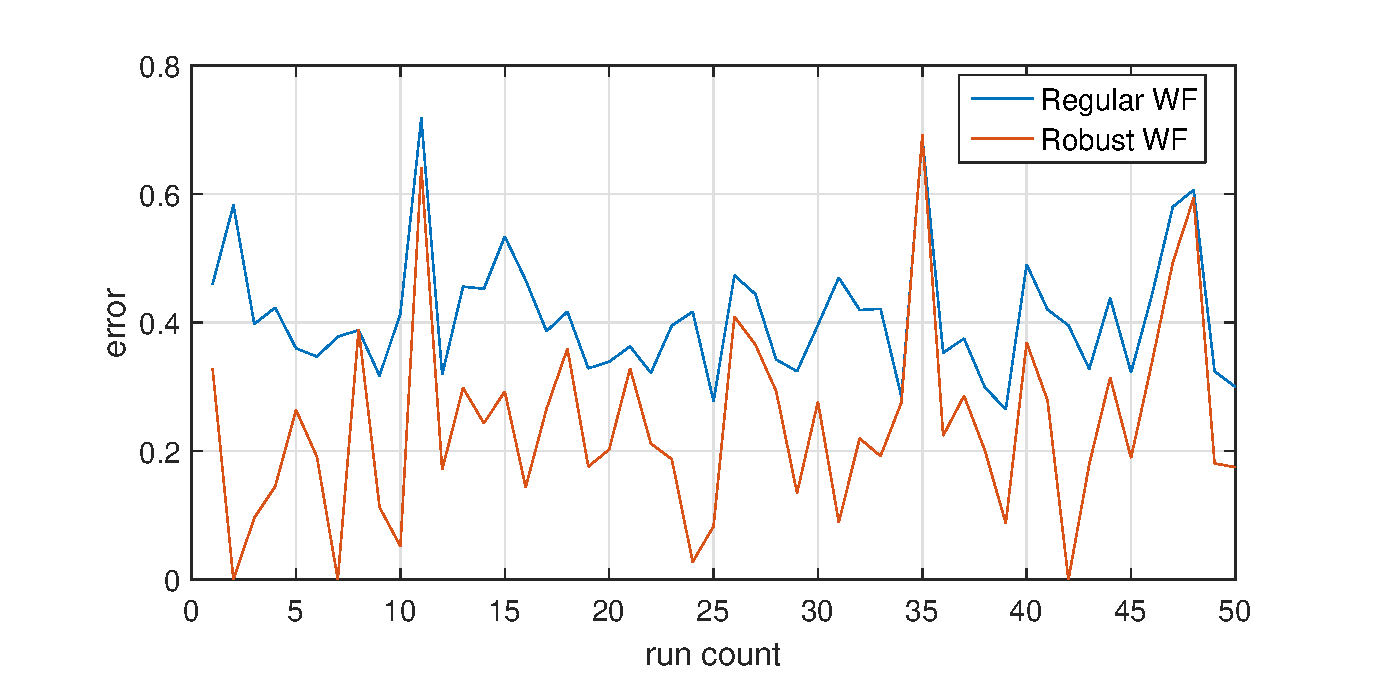
\includegraphics[width=\textwidth]{figs/snr_5db}
         \caption{SNR = 5dB}
         \label{fig:y equals x}
     \end{subfigure}
     \hfill
     \begin{subfigure}[b]{0.75\textwidth}
         \centering
         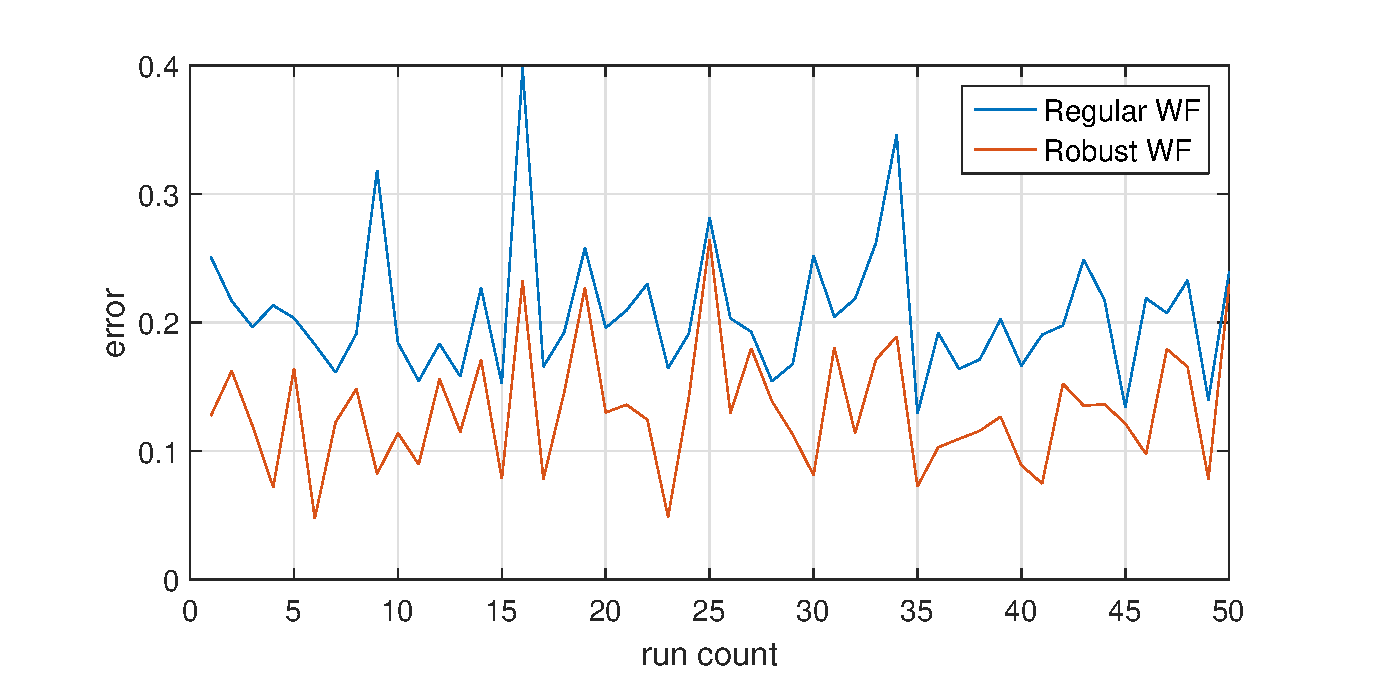
\includegraphics[width=\textwidth]{figs/snr_10db}
         \caption{SNR = 10dB}
         \label{fig:three sin x}
     \end{subfigure}
     \hfill
     \begin{subfigure}[b]{0.75\textwidth}
         \centering
         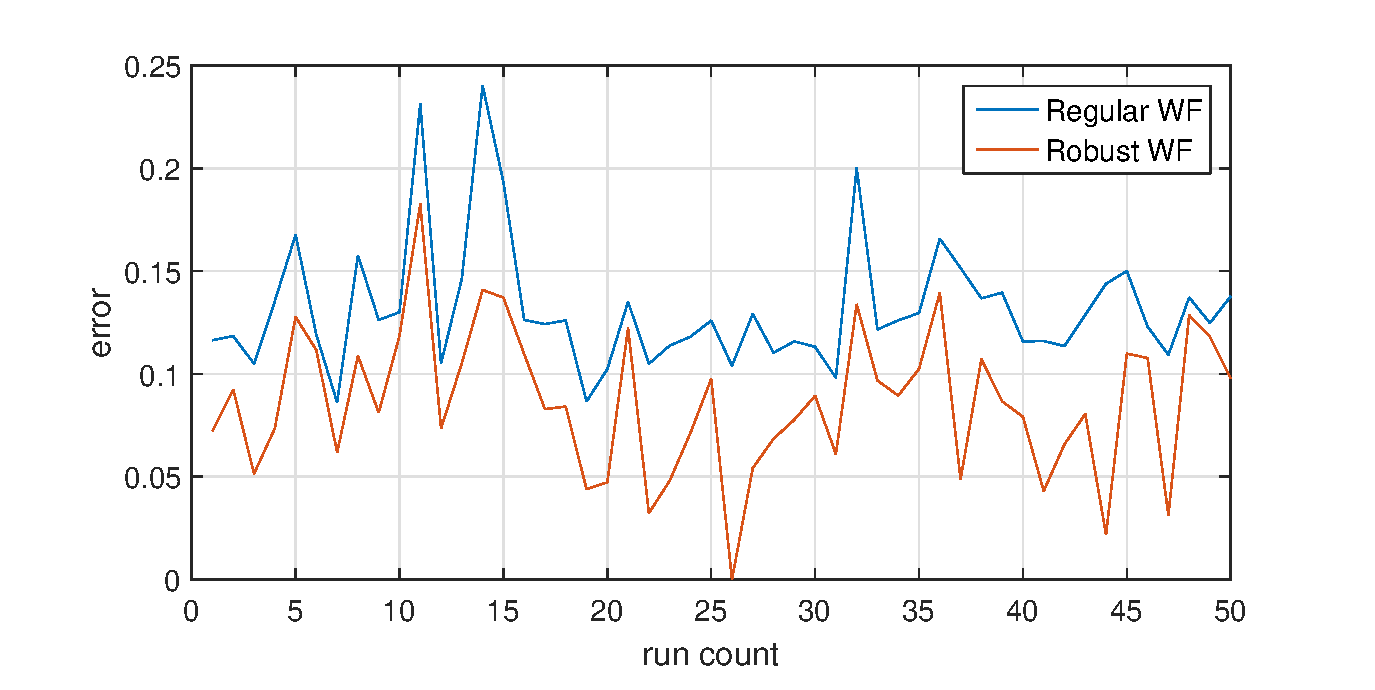
\includegraphics[width=\textwidth]{figs/snr_15db}
         \caption{SNR = 15dB}
         \label{fig:five over x}
     \end{subfigure}
 \end{figure}
 
 \begin{figure}  \ContinuedFloat
 \centering 
     \begin{subfigure}[b]{0.75\textwidth}
         \centering
         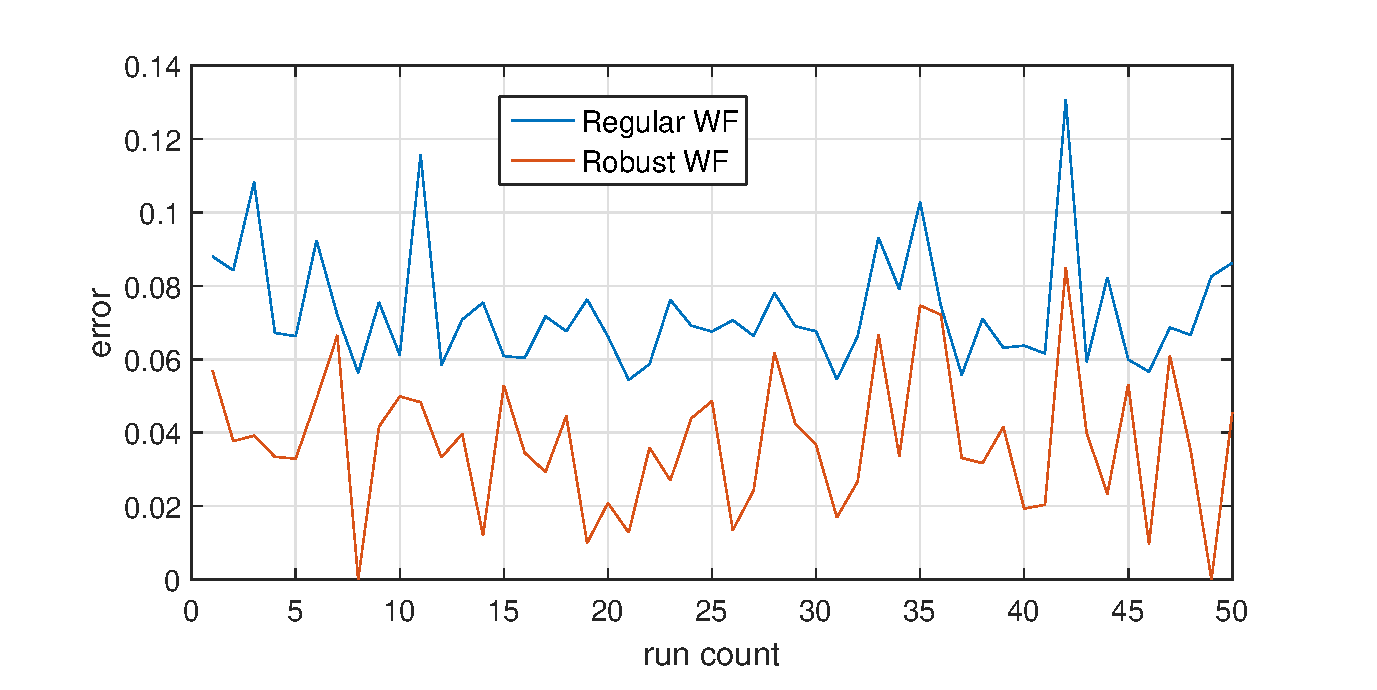
\includegraphics[width=\textwidth]{figs/snr_20db}
         \caption{SNR = 20dB}
         \label{fig:five over x}
     \end{subfigure}
     \hfill
     \begin{subfigure}[b]{0.75\textwidth}
         \centering
         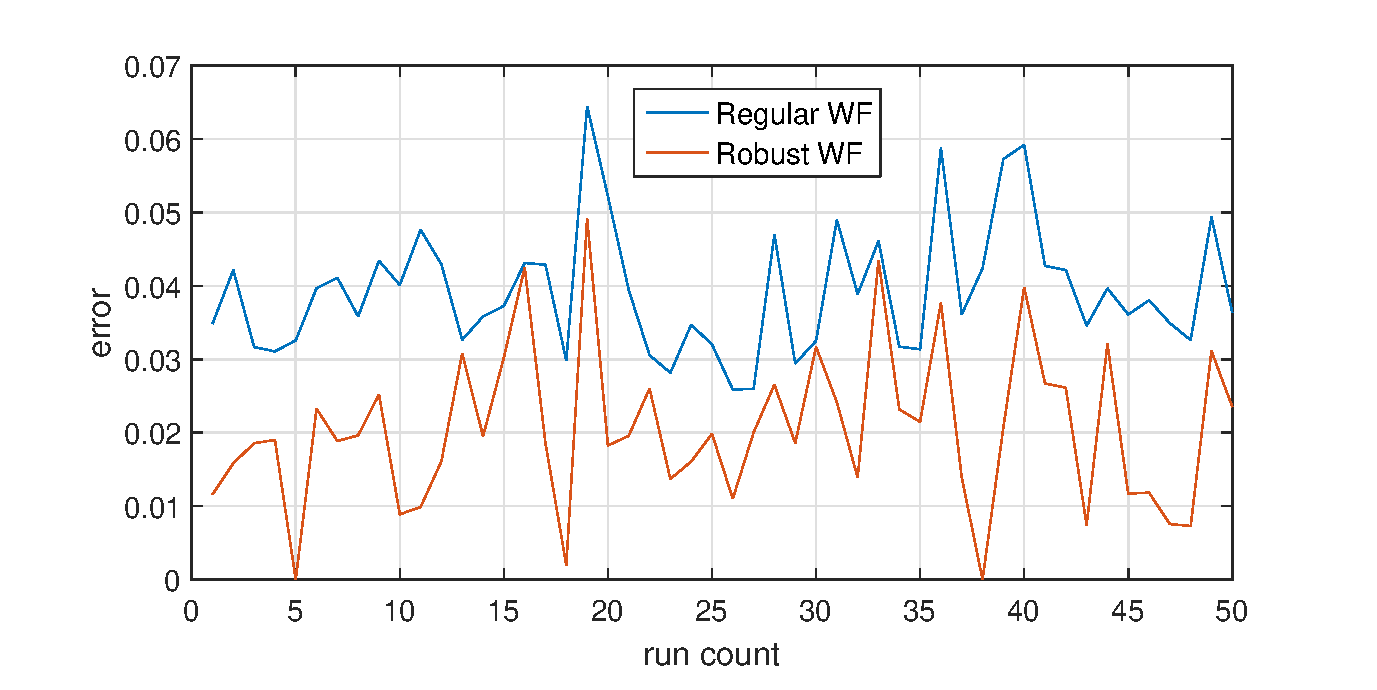
\includegraphics[width=\textwidth]{figs/snr_25db}
         \caption{SNR = 25dB}
         \label{fig:five over x}
     \end{subfigure}
     \hfill
     \begin{subfigure}[b]{0.75\textwidth}
         \centering
         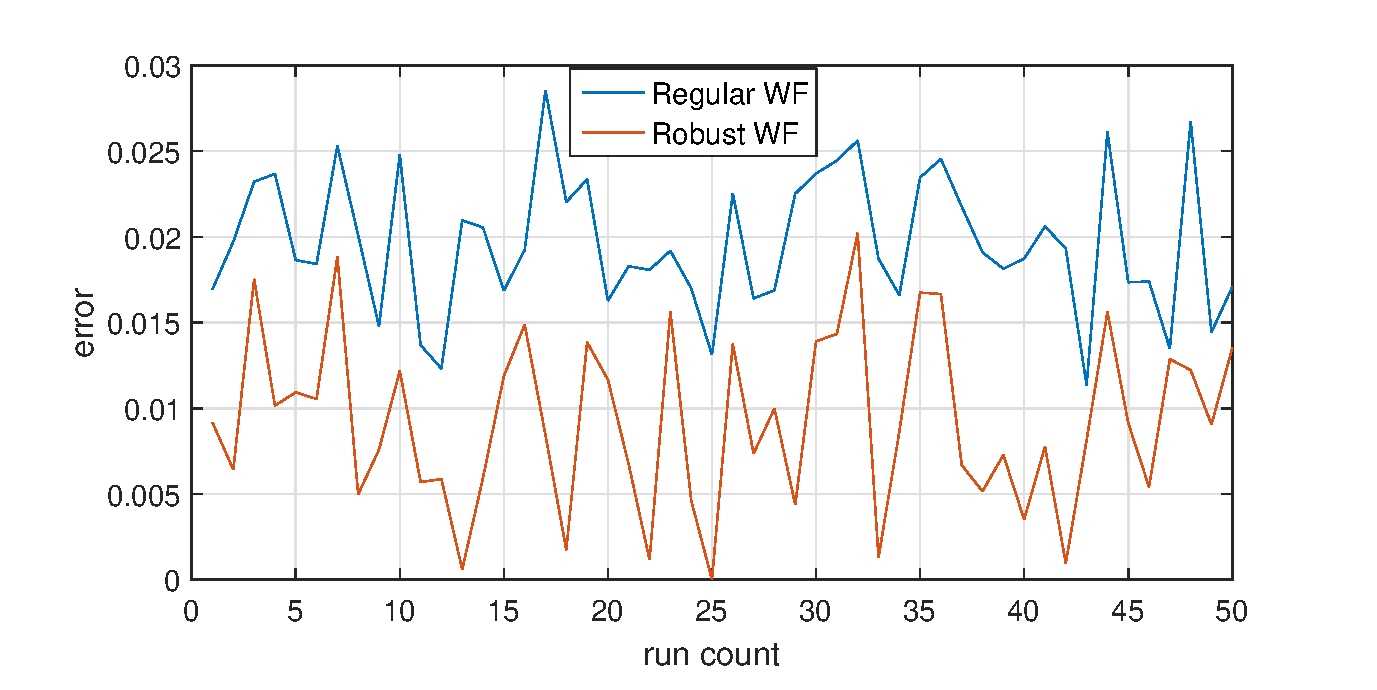
\includegraphics[width=\textwidth]{figs/snr_30db}
         \caption{SNR = 30dB}
         \label{fig:five over x}
     \end{subfigure}


        \caption{error $e$ for Robust versus Regular Wirtinger flow algorithm in $50$ runs}
        \label{fig_sim}
\end{figure}




To get a sense on improvement in SNR (dB) we take the average of errors in all runs and compare the two algorithm in different SNRs.
By looking at the table \ref{table:1}, we can see that adding code constraints to WF algorithm reduces the error to almost half of regular WF.
In terms of SNR, there is almost 5dB gain advantage in implementing robust WF against regular WF.
 \begin{table}
  \centering
\caption {Average error $e = \parallel \mathbf{x}_1 - \hat{\mathbf{x}}_1 \parallel_2$ for $50$ runs }
\label{table:1}
 \begin{tabular}{ p{1cm}|p{2.5cm}|p{2.5cm}  }
 %\hline
 %\multicolumn{4}{|c|}{Decoder Saving} \\
%\hline
SNR & Regular WF& Robust WF\\
 \hline
 
 30   &   0.196     & 0.0092   \\
 \hline
 25   &   0.393  &  0.0205\\
 \hline
 20   &   0.073     & 0.0374\\
 \hline
 15   &   0.1263    & 0.069\\
  \hline
 10   &   0.2067    & 0.1317\\
 \hline
 5   &   0.4093  & 0.2414\\

\end{tabular}
\end{table}

We also need to make sure that imposing code constraint on the signal of interest $\mathbf{x}_1$, would not make the error on other signals worst. 
Our simulations show that in every instance the error stays the same in other signals or slightly better. However, the main advantage would be in the signal that code constraint
would be imposed on it.


















